\documentclass[11pt]{article}

\usepackage[letterpaper,margin=0.82in]{geometry}
\usepackage[T1]{fontenc}
\usepackage[utf8]{inputenc}
\usepackage{mathptmx}
\usepackage{microtype}
\usepackage{amsmath,amssymb,bm,amsthm}
\usepackage{booktabs,graphicx}
\usepackage[numbers,sort&compress]{natbib}
\usepackage[hidelinks]{hyperref}

\graphicspath{{../figures/}}
\newtheorem{theorem}{Theorem}
\newtheorem{proposition}{Proposition}
\newtheorem{corollary}{Corollary}
\newcommand{\E}{\mathbb E}
\newcommand{\R}{R^{\mathrm{tot}}}
\DeclareMathOperator{\tr}{tr}

\title{Credit covariance and routing in dendritic trees}
\author{Houman Safaai, Maceo Richards, and Bernardo L. Sabatini}
\date{}

\begin{document}
\maketitle

\begin{abstract}
Biological learning must transform a small number of cellular teaching signals
into distinct updates at many synapses. We formulate this as a constrained
routing problem. In a directed conductance-based dendritic tree, each exact
synaptic gradient separates into a synapse-local eligibility and a somatic
error transported through the unique path to that synapse. A feedback circuit
therefore chooses both a coordinate, such as neuron identity, and a routing
subspace over compartments. We define credit capture as the gradient energy in
that subspace and show that it determines a one-step descent guarantee. Across
a task distribution, the relevant object is the covariance of exact credit,
not feedback rank alone: the optimal unconstrained channels are covariance
eigenvectors, whereas biological channels are restricted to ancestry-supported
routes. Conductance regulates the gain of those routes, and focal inhibition
attenuates descendants selectively at fixed state. The theory predicts that
learning succeeds when task-credit covariance aligns with the anatomical route
dictionary and that route overlap controls interference. These results define
a communication-level theory linking local plasticity, dendritic topology and
task structure.
\end{abstract}

\section{Introduction}

Credit assignment asks how an outcome-dependent teaching signal can produce
the parameter-specific changes required for learning. Backpropagation solves
this problem by communicating one derivative to every parameter
\citep{rumelhart1986learning}. Biological synapses instead update from signals
available locally, motivating three-factor plasticity, feedback alignment and
dendritic learning theories
\citep{fremaux2016threefactor,richards2019dendritic,lillicrap2020backprop}.
Most formulations specify how a neuron receives an error but do not specify
how that error is addressed across a branched dendritic tree.

We distinguish three objects. A \emph{teaching coordinate} identifies which
neuron or functional population should change. A \emph{route} determines which
compartments within that neuron share the coordinate. A synapse-local
\emph{eligibility} converts the routed signal into a conductance update. This
separation makes feedback bandwidth, dendritic topology and conductance
comparable within one formalism.

The theory has four parts. First, exact differentiation of a directed
conductance tree identifies the information required at each synapse. Second,
we treat restricted feedback as projection into a route subspace and relate
projection energy to descent. Third, we replace a single gradient by its task
distribution and obtain a covariance-matching objective. Finally, we derive
consequences for inhibitory route gain and task interference. The claims
concern communication and local learning; they do not
assert that a particular biological circuit computes oracle projection
coefficients.

\section{Exact credit in a conductance tree}

Consider a directed rooted tree. Compartment $n$ receives synapses
$i\in\mathcal S_n$ and child compartments $c\in\mathcal C_n$. Its steady-state
voltage is
\begin{equation}
V_n=R_n^{\mathrm{tot}}
\left(\sum_{i\in\mathcal S_n}g_i x_iE_i+
\sum_{c\in\mathcal C_n}g_{c\to n}^{\mathrm{den}}a_c+g_n^LE_L\right),
\quad
R_n^{\mathrm{tot}}=(g_n^{\mathrm{tot}})^{-1},
\label{eq:voltage}
\end{equation}
where $a_c=f_c(V_c)$ and total conductance includes leak, active synaptic
conductance and child coupling.

\begin{theorem}[Local eligibility and transported error]
For a loss $\mathcal L$ that depends on the root output, the gradient of a
synaptic conductance $g_i$ at compartment $n$ is
\begin{equation}
\frac{\partial\mathcal L}{\partial g_i}
=\underbrace{x_iR_n^{\mathrm{tot}}(E_i-V_n)}_{e_i\text{, local eligibility}}
\underbrace{\frac{\partial\mathcal L}{\partial V_n}}_{\delta_n\text{, compartment error}}.
\label{eq:factorization}
\end{equation}
If neuron $u$ has somatic error $\delta_{0,u}$, then
\begin{equation}
\delta_n=\delta_{0,u}\widetilde\alpha_n,
\qquad
\widetilde\alpha_n=
\prod_{(j\to k)\in\operatorname{path}(n\to0)}
f_j'(V_j)R_k^{\mathrm{tot}}g_{j\to k}^{\mathrm{den}}.
\label{eq:pathgain}
\end{equation}
\end{theorem}

Equation~\ref{eq:factorization} follows by differentiating the numerator and
denominator of Eq.~\ref{eq:voltage}; the driving-force term $E_i-V_n$ is the
conductance-specific contribution. Equation~\ref{eq:pathgain} follows by
iterating the child-to-parent derivative along the unique path. Thus an exact
gradient requires a local eligibility, a neuron-specific somatic coordinate
and path-dependent transport. A global scalar broadcast removes the second and
third objects simultaneously. Neuron-indexed feedback restores the coordinate;
exact local path factors would then restore the remaining compartment field.

Numerical reconstruction of Eqs.~\ref{eq:factorization}--\ref{eq:pathgain}
matches automatic differentiation to below $2\times10^{-7}$ maximum relative
error across the archived diagnostic cohort (Fig.~\ref{fig:feedback}a). In
regular $[3,3]$ trees, preserving neuron identity raises the cosine between
available and exact dendritic gradients from approximately zero to 0.708 in
conductance-based trees and 0.625 in matched additive trees
(Fig.~\ref{fig:feedback}b,c). Exact path transport makes the theorem-derived
eligibility sufficient to match the same-architecture backpropagation
reference (Fig.~\ref{fig:feedback}d).

\begin{figure}[t]
\centering
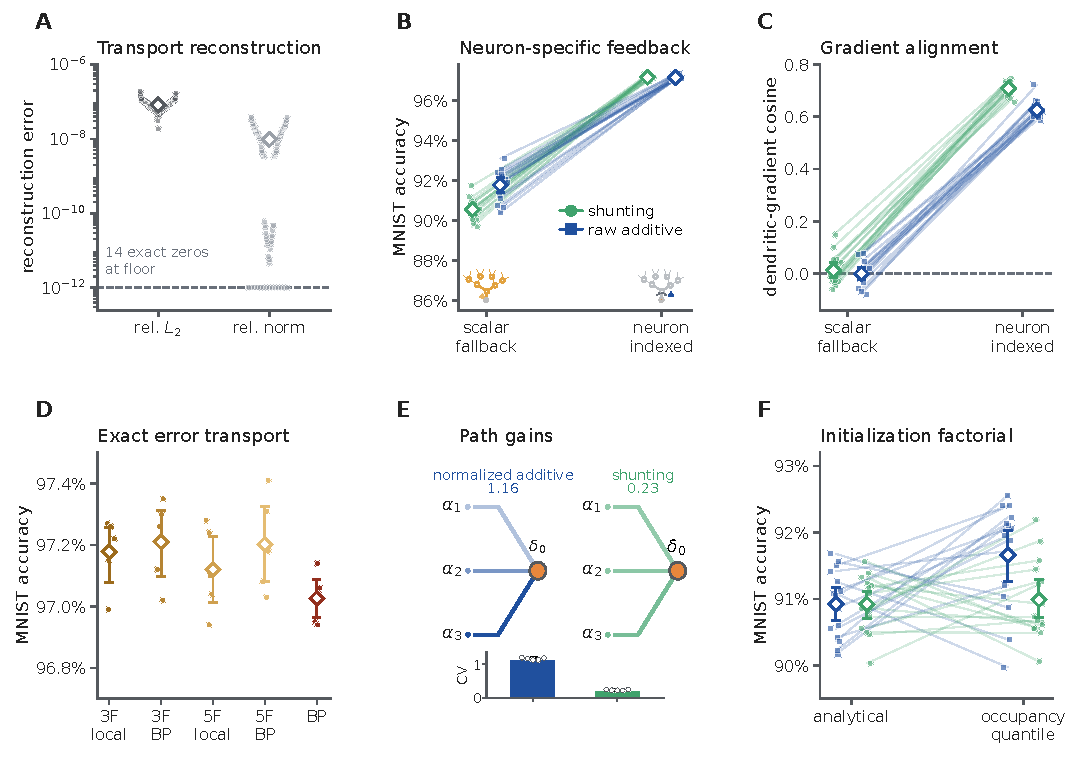
\includegraphics[width=\textwidth]{main/figure_02_panels_A-F.pdf}
\caption{\textbf{The principal feedback limitation is loss of teaching-signal
identity.} Exact analytic gradients agree with automatic differentiation
(\textbf{A}). Neuron-indexed feedback improves both learning and gradient
direction relative to scalar fallback (\textbf{B,C}). Exact transport isolates
the local eligibility (\textbf{D}); the remaining panels separate conductance
operating point, initialization and one-step optimization. This figure is
shared with the comprehensive working draft and would be redrawn or assigned
to only one paper before independent submission.}
\label{fig:feedback}
\end{figure}

\section{Feedback as a route subspace}

Let $A_T\in\{0,1\}^{p\times q}$ be the synapse-by-route ancestry matrix of
tree $T$: $(A_T)_{ik}=1$ when route site $k$ lies between synapse $i$ and the
soma. With local or anatomical weights $W_e$, route gains $\bm\beta$ and a
channel assignment $C$, an $m$-channel feedback vector $\bm z$ generates
\begin{equation}
\widehat{\bm g}=D_T\bm z,
\qquad D_T=W_eA_T\operatorname{diag}(\bm\beta)C.
\label{eq:dictionary}
\end{equation}
Topology fixes support. Conductance changes gains and conditioning but cannot
create an ancestry relation absent from $A_T$.

Let $W\succ0$ be diagonal, $\overline{\bm g}=W^{1/2}\bm g$ and
$\overline D=W^{1/2}D_T$. Denote by $P_D$ the Euclidean orthogonal projector
onto $\operatorname{col}(\overline D)$. Define
\begin{equation}
R(T,\bm g;W)=
\frac{\lVert P_D\overline{\bm g}\rVert_2^2}
{\lVert\overline{\bm g}\rVert_2^2}.
\label{eq:capture}
\end{equation}

\begin{theorem}[Capture and one-step descent]
Let $\overline{\mathcal L}$ have $L_W$-Lipschitz gradient in the transformed
coordinates. For $0<\eta<2/L_W$,
\begin{equation}
\overline{\mathcal L}(\overline{\bm w}-\eta P_D\overline{\bm g})
\leq \overline{\mathcal L}(\overline{\bm w})-
\eta\left(1-\frac{L_W\eta}{2}\right)
\lVert P_D\overline{\bm g}\rVert_2^2.
\label{eq:descent}
\end{equation}
At $\eta=1/L_W$, the projected-to-full-gradient descent guarantees have ratio
$R(T,\bm g;W)$.
\end{theorem}

The proof is the descent lemma followed by
$\overline{\bm g}^{T}P_D\overline{\bm g}=\lVert P_D\overline{\bm g}\rVert^2$.
Ten thousand random positive-definite quadratic trials produced no bound
violations; the minimum numerical slack was $2.67\times10^{-7}$ and the capture
identity agreed to $1.89\times10^{-15}$. The theorem is a one-step statement
for an exact gradient expressed in declared coordinates. It does not show that
a circuit can infer the least-squares coefficients $\bm z$.

\section{Task distributions select useful routes}

A single gradient cannot determine whether a route dictionary will be useful
over learning. Let
$C_g=\E[\overline{\bm g}\,\overline{\bm g}^{T}]$ be the uncentered covariance
of exact task credit. We define energy-weighted expected capture as the ratio
of expected projected and total energy.

\begin{theorem}[Covariance matching]
For a fixed route subspace,
\begin{equation}
R(T,C_g)=\frac{\tr(P_D C_g)}{\tr(C_g)}.
\label{eq:covariance}
\end{equation}
\end{theorem}

\begin{corollary}[Unconstrained upper bound]
Among all $m$-dimensional subspaces, Eq.~\ref{eq:covariance} is maximized by the
leading $m$ eigenvectors of $C_g$. The maximum is
$\sum_{j=1}^{m}\lambda_j(C_g)/\tr(C_g)$.
\end{corollary}

The corollary is the Ky Fan maximum principle. It separates channel count from
basis choice. A rank-$m$ PCA dictionary is an unconstrained information oracle;
an ancestry dictionary is restricted to nested biological supports. The
relevant comparison is therefore not whether exact credit is low rank, but how
much task covariance lies in the route subspace available to the cell.

This condition explains both success and failure. When exact gradients are
constructed with a fraction $a$ of their energy in a fixed eight-route
MICrONS subspace, measured capture equals $a$ and predicts one-step and
iterative loss progress (Fig.~\ref{fig:alignment}). When gradients are derived
from a small measured visual-response cohort without imposing alignment,
morphology does not reliably exceed ancestry-shuffled routes. Anatomical
capacity is therefore not evidence of task alignment.

\begin{figure}[t]
\centering
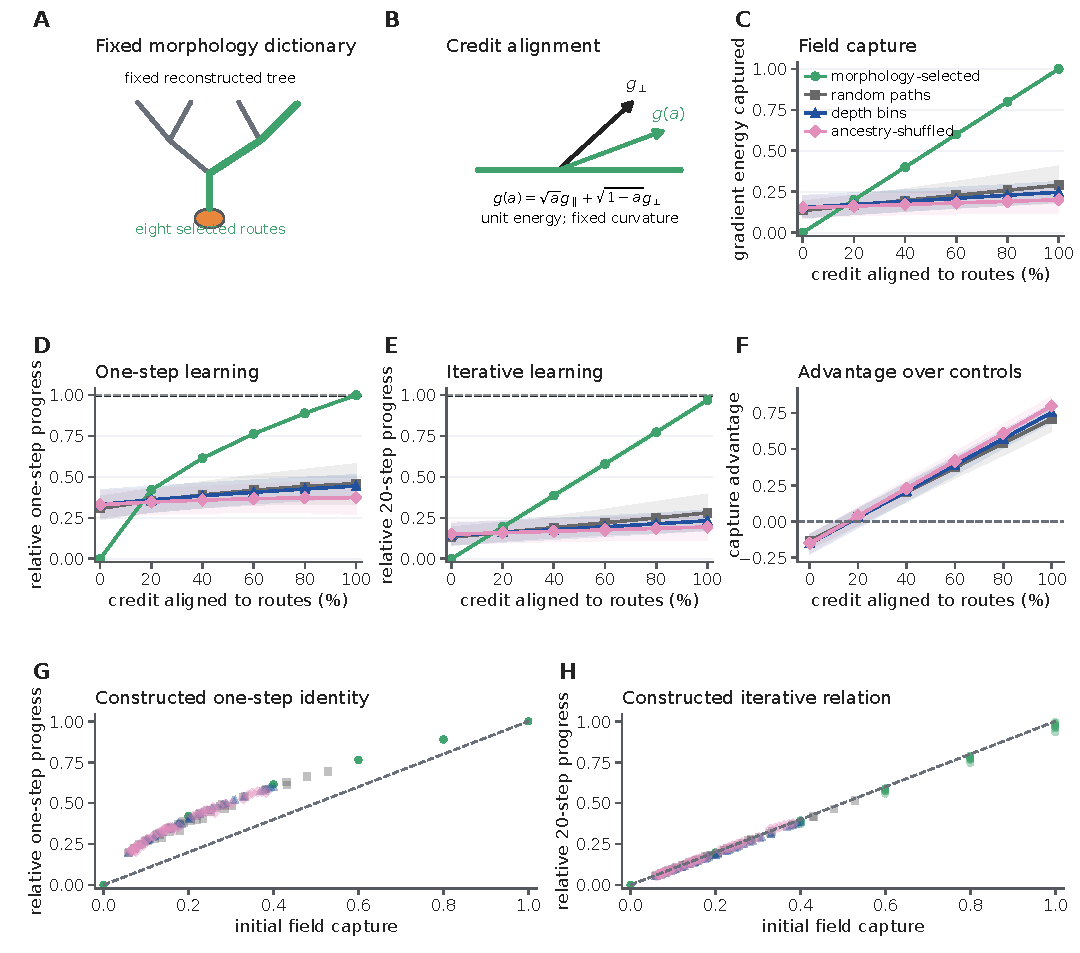
\includegraphics[width=\textwidth]{supplementary/figure_S05_panels_A-H.pdf}
\caption{\textbf{Route value is conditional on task-credit alignment.}
Controlled gradients interpolate between the route span and its orthogonal
complement at fixed total energy. Capture and optimization progress rise with
imposed alignment, whereas structural controls do not receive this advantage.
This controlled construction establishes sufficiency, not biological use of
the oracle coefficients.}
\label{fig:alignment}
\end{figure}

\section{Conductance provides descendant-selective gain control}

Let $\alpha_n^{\mathrm{cond}}$ be Eq.~\ref{eq:pathgain} without reactivation
derivatives. At fixed forward state and fixed coupling conductances, add
inhibitory conductance $\Delta G_k^I\geq0$.

\begin{proposition}[Fixed-state shunting selectivity]
\begin{equation}
\frac{\alpha_n^{\mathrm{cond}}(\Delta G^I)}
{\alpha_n^{\mathrm{cond}}(0)}=
\prod_{k\in\mathcal A(n)}
\frac{g_k^{\mathrm{tot}}}{g_k^{\mathrm{tot}}+\Delta G_k^I},
\quad
\frac{\partial\log\alpha_n^{\mathrm{cond}}}{\partial G_k^I}=
\begin{cases}
-R_k^{\mathrm{tot}},&k\in\mathcal A(n),\\
0,&k\notin\mathcal A(n),
\end{cases}
\label{eq:shunt}
\end{equation}
where $\mathcal A(n)$ is the path from $n$ to the soma.
\end{proposition}

Thus a focal conductance change attenuates a nested descendant domain. The
result does not imply that inhibition improves learning: if $z_n=\log\alpha_n$
and the attenuation is $\beta_n$, then
$\operatorname{Var}(z-\beta)=\operatorname{Var}(z)+\operatorname{Var}(\beta)
-2\operatorname{Cov}(z,\beta)$. Gain dispersion narrows only when the
attenuation covaries sufficiently with the original gain. Shunting is a
route-gain operator, not a universal gradient preconditioner.

\section{Route overlap predicts interference}

Let Task A be at a local quadratic optimum with Hessian $H_A\succeq0$. A Task-B
update routed by $M_B$ is $-\eta M_B\bm g_B$. Exact expansion gives
\begin{equation}
\Delta\mathcal L_A=
\frac{\eta^2}{2}\bm g_B^T M_B^T H_A M_B\bm g_B.
\label{eq:interference}
\end{equation}
For equal-size routes with fractional overlap $\omega$, opposing requested
updates on shared coordinates and off-route leakage $\lambda$, the normalized
loss increase is
\begin{equation}
\Delta\mathcal L_A=\frac{\eta^2}{2}
\left[4\omega+\lambda^2(1-\omega)\right].
\label{eq:simpleinterference}
\end{equation}
The identity makes two independent failure modes explicit: reuse of the same
route by incompatible tasks and leakage outside the requested route. Numerical
evaluation agrees with explicit vector updates to $4.16\times10^{-17}$ maximum
absolute error (Fig.~\ref{fig:interference}). It is static and does not model
spiking, eligibility timing or consolidation.

\begin{figure}[t]
\centering
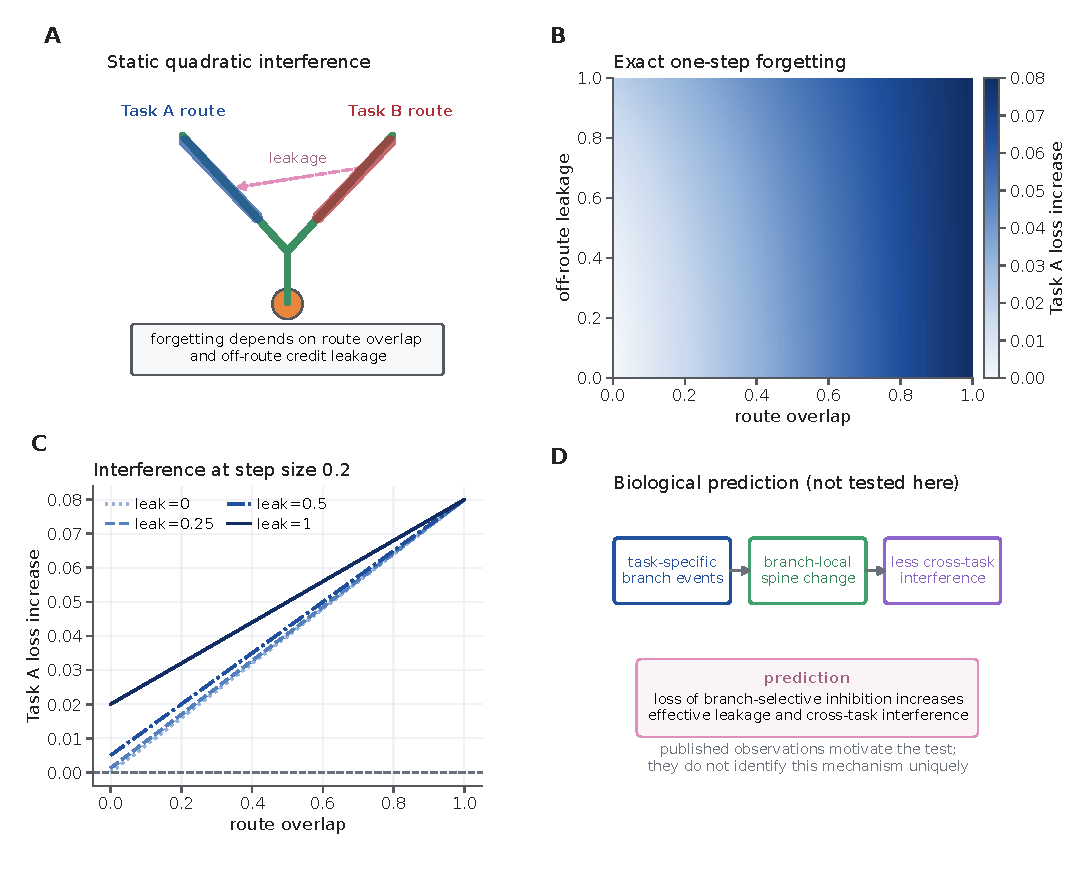
\includegraphics[width=0.88\textwidth]{supplementary/figure_S06_panels_A-D.pdf}
\caption{\textbf{Overlap and off-route leakage determine one-step
interference.} The heat map evaluates Eq.~\ref{eq:simpleinterference}; line
slices show how anatomical route reuse and imperfect feedback make separable
contributions. The biological link is a prediction, not a causal test.}
\label{fig:interference}
\end{figure}

\section{Discussion}

The main result is a change in the level at which local credit assignment is
posed. A cellular teaching signal is not merely too small or noisy. It must be
addressed. Neuron identity supplies a coarse coordinate; dendritic ancestry
expands it into nested supports; local eligibility resolves synapse-specific
sign and scale; conductance regulates route gain. This decomposition connects
three-factor plasticity to an explicit communication problem.

The covariance formulation prevents two common overinterpretations. First,
low rank is not sufficient: an unconstrained singular vector need not be
implementable by a dendritic route. Second, anatomical route capacity is not
task relevance. The same tree can be well suited to one credit covariance and
poorly aligned with another. Negative task-alignment results are therefore a
boundary of the theory rather than a contradiction.

The framework yields experimentally separable predictions. Teaching signals
should preserve neuron identity before resolving within-tree location. Focal
conductance changes should alter plasticity preferentially in descendant
domains when somatic output is controlled. Tasks that recruit overlapping
routes should interfere more strongly. Testing these predictions requires
longitudinal, branch-resolved learning data;
the present mathematics alone does not identify a biological implementation.

\section{Methods and numerical checks}

All projections use an explicit weighted coordinate transformation before
ordinary Euclidean least squares. Capture is the ratio of projected to total
energy, not the mean of unweighted sample-wise cosines. The descent theorem was
verified on 10,000 random positive-definite quadratics at $\eta=1/L_W$. The
interference surface used 101 values each of $\omega$ and $\lambda$ and was
checked against explicit vector updates. Regular-tree numerical diagnostics,
controlled alignment experiments and route-interference controls use the
frozen tables and code documented in the comprehensive project repository.

\section*{Data and code availability}

This working companion draft uses only derived source tables and scripts in the
parent journal project. A separate archival release and a non-overlapping
figure set would be prepared before submission.

\section*{Competing interests}

The authors declare no competing interests.

\bibliographystyle{unsrtnat}
\bibliography{../references}

\end{document}
